\chapter{Kalman Filter Modelling and Design}

The low update rate of the object detector (as mentioned in Subsection~\ref{ssec:meth_nn_performance_increase}) necessitated the use of a Kalman Filter to both increase the reliability of the measurements and to get a better estimate of the objects state in between measurements.

There were a number of design decisions which had to be made when modelling the system and implementing the filter. These are discussed in this chapter, as well as some simulation and testing results.


\section{System modelling}
A Kalman Filter (KF) was used to estimate the state of the tracked object as it moved around. Since the camera system generally rotates around an axis and there is no reliable estimate of the distance from the camera to the object being tracked, it was decided that the state would be measured in absolute angular coordinates.

A model of the dynamics of the tracked object had to be chosen for the KF to operate optimally. However, there is no possible "correct" model for the movements of the object being tracked (for example, a cheetah won't stick to the rule of moving at a constant velocity) and no way to estimate the disturbances $u$ which may effect its decision to change its velocity. Thus, it was decided that the model would make the incorrect assumption the the object would either maintain a constant velocity, constant acceleration of exponentially decaying acceleration. These three approaches needed to be tested, with the best being used in the final model.

This resulted in the global angular position, velocity and acceleration of the tracked object being estimated. These were stored in the state matrix $x$ as,

\[ \underline{x} = \begin{bmatrix} \theta \\ \dot{\theta} \\ \ddot{\theta} \end{bmatrix} \]

These states are related through integration, where $\theta = \int{\dot{\theta} dt} = \int{\int{\ddot{\theta} dt}dt}$. They can be approximated using the discrete integration formulae, $\dot{\theta}_k = \dot{\theta}_{k-1} + \Delta T \ddot{\theta}_{k-1}$ and $\theta_k = \theta_{k-1} + \Delta T \dot{\theta}_{k-1}$. The prediction matrix was thus chosen as,

\[ F = \begin{bmatrix} 1 & \Delta T & 0 \\
                       0 & 1 & \Delta T \\
					   0 & 0 & \beta
		\end{bmatrix} \]

where $\beta$ is a factor which could be $\beta = 1$ for constant acceleration ($a_i = a_{i-1}$ in the predict stage), $0 < \beta < 1$ for decaying accelerating (for example, $a_i = 0.9 a_{i-1}$) or $\beta = 0$ for no acceleration. This was done to ensure quick and easy prototyping.

Next, the sensor needed to be added. The neural network returns the coordinates of the position of the object, measured in pixels. For the sake of modularity and simpler math, the pixel range of \pyth{pixel} $\in$ \pyth{[0, 299]} along a single axis was normalized to a value \pyth{pixel_norm} $\in$ \pyth{[-1, 1]}, with a pixel value of zero corresponding to the centre of the image. An illustration of this is shown below, in Figure~\ref{fig:pixel_to_angle}.

\begin{figure}[h!]
  \centering
  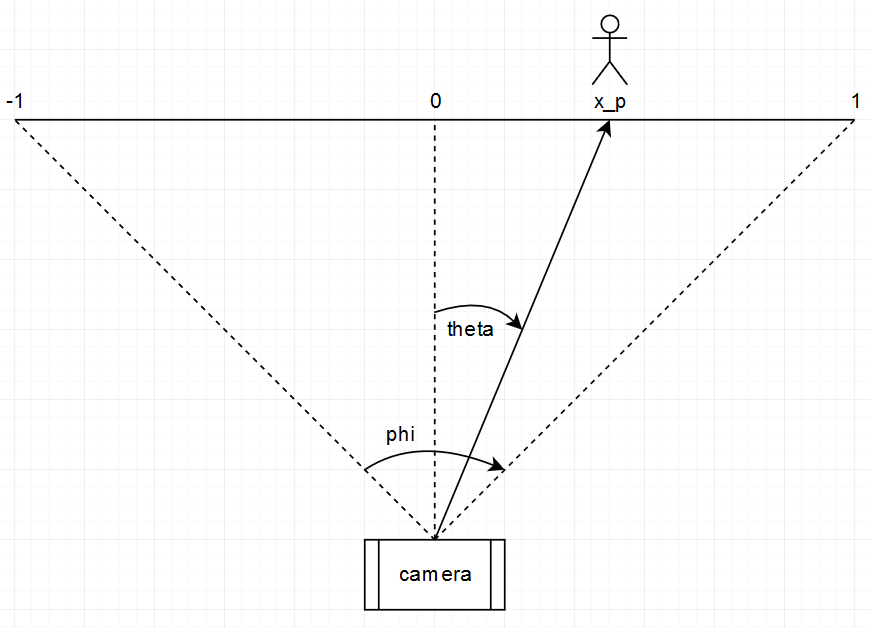
\includegraphics[width=\textwidth]{methodology/pixel_to_angle2}
  \caption{\label{fig:pixel_to_angle} Diagram showing the mapping from normalized pixel to angle.}
\end{figure}

Note that the pixel coordinate of the detected object is given by \pyth{x}, the angle to the object is \pyth{phi} ($\phi$) and the field of view of the camera is \pyth{theta} ($\theta$). Letting the distance between the camera and the plane at the closest point be noted as $L$, one can convert between pixel and angle as follows:

\[ L = \frac{1}{\tan{\theta/2}} = \frac{x}{\tan{\phi}} \]
Resulting in,
\[ \phi = \tan^{-1}{\left( x\cdot{}\tan{ \theta/2 } \right) }
\qquad or
\qquad x = \frac{\tan{\phi}}{\tan{\theta/2}} \]
%\phi = \tan^{-1}{\left( \frac{\tan{ \theta/2 }}{x} \right) }

A plot of this function is shown in Figure~\ref{fig:pixel_to_angle_plot}. Clearly, the mapping from pixel to angle is nonlinear.

\begin{figure}[h!]
  \centering
  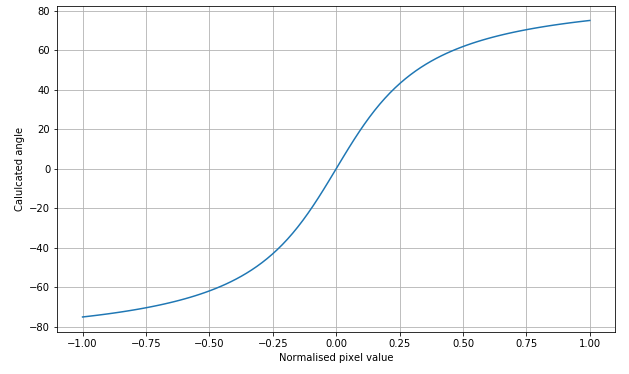
\includegraphics[width=\textwidth]{methodology/pixel_to_angle_plot}
  \caption{\label{fig:pixel_to_angle_plot}Plot showing the mapping from normalized pixel to angle.}
\end{figure}

For this reason, an EKF was considered instead of a linear Kalman Filter - a one pixel error in the middle of the image will propagate to a different angular error than a one pixel error at the edge. The Jacobian could then be calculated as,

\[ \frac{\delta h}{\delta x} = \frac{\delta}{\delta x} \left[ \frac{\tan{\phi}}{\tan{\theta/2}} \right] = \frac{1 + \tan{(\phi)}^2}{\tan{\theta/2}} \]

However, for reasons explained in Section \ref{sec:kf_implementation}, both the KF and EKF were considered.

Next, the $Q$ and $R$ matrices needed to be determined. In most systems, these can be calculated after careful modelling of the objects dynamics and consultation with component datasheets. However, in this system, the $Q$ matrix determined for an object which is close to the camera would be wildly inaccurate when the object is farther away, since distance affects the perceived angular movement of an object moving in a straight line. Since there is no distance estimate, this could not be reliably factored into a constantly changing $Q$. In addition, the neural network has no obvious value to use for the sensor noise, $R$.

What is known, however, is how process uncertainty in the acceleration and velocity of the model would propagate to the the other states. Thus, the following structure was decided for the process uncertainty matrix $Q$:
\[ Q = \begin{bmatrix}
	Q_a \frac{\Delta t^2}{2} & 0 & 0 \\
	0 & Q_a \Delta t & 0 \\
	0 & 0 & Q_a \end{bmatrix} \]

Thus, $Q_a$ (the maximum amount of deviation from the acceleration model) and R were left  parameters to be tuned using recorded data.

\section{Implementation of the Kalman Filter algorithm}

While python wasn't designed for purely numerical programming (such as matrix multiplication), when the correct packages are used it can approach C-level speeds. \pyth{numpy} is one such package - it provides python bindings to C arrays, resulting in incredible speedups over regular python arrays.

The Kalman Filter and Extended Kalman Filter were implemented as python classes which contain \pyth{numpy} matrices. The code can be found on the authors \href{https://github.com/alknemeyer/EEE4022S-Thesis-Project/blob/master/Final%20code/extended_kalman_filter.ipynb}{GitHub repository.} \\

\subsection{Timing issues due to sampling time inconsistencies}
Kalman Filters usually operate in control systems with constant loop times. However, due to the fact that the object detection pipeline had a variable amount of time between samples, the Kalman Filters time parameters (found in the $F$ and $Q$ matrices) needed to be continuously updated based on the actual amount of time that had passed since the last predict/update cycle.

This time stamp was also used to get a state estimate from the Kalman Filter between updates from the object detector.

Pseudo code which performs these operations is shown below.\\

\begin{python}
def update(measurement, previous_time):
	time = get_current_time()
	new_T = time - previous_time
	previous_time = time
	
	# update the time-dependant parameters
	new_F, new_Q = update_F_and_Q(new_T)
	
	predict(new_F, new_Q) # make predictions for x, P
	update(new_F, measurement) # compare to measurement

def estimate_current_position():
	time = get_current_time()
	temp_T = time - previous_time
	new_F, _ = update_F_and_Q(new_T)
	
	return new_F * x
\end{python}

\subsection{Tuning the process noise and sensor uncertainty}
The next step was to find and set reasonable values for the process noise $Q$ and sensor uncertainty $R$. This was doing by running the computer vision algorithm while a human walked and ran around the lab. The results of this were saved to a file, allowing for easy offline simulation. A plot of the raw updates from the neural network are shown below, in Figure~\ref{fig:raw_nn_results}.

\begin{figure}[h!]
  \centering
  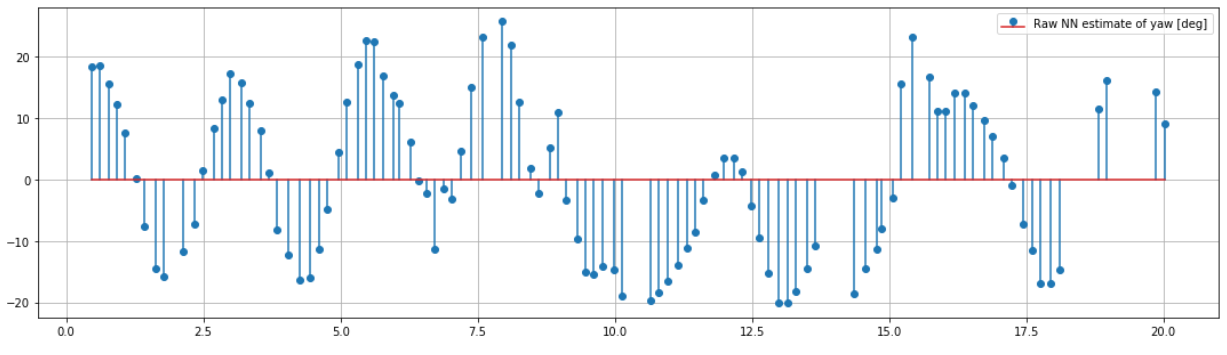
\includegraphics[width=\textwidth]{methodology/raw_nn_results}
  \caption{\label{fig:raw_nn_results} A plot showing the outputs of the neural network, and the timing thereof.}
\end{figure}

Note how the time between inferences from the neural network is not constant - while all of the calculations in the neural network are the same in each run, non-constant run times are the natural consequence of running a control loop on a non real time operating system.

In addition, there are times when a few hundred milliseconds pass without receiving a new update - this occurs when the neural network can't find an object in the frame. It is worth noting that the neural network is in fact very good at locating objects, and misses them infrequently. However, the frequent and large gaps in object locations was added in order to simulate tracking an object which may disappear behind a bush or some other obstacle.

Next, a small script was made to speed up the trial-and-error process of comparing the advantages and disadvantages of a variety of $Q$ and $R$ values. In addition, the possibility of switching to a Kalman Filter and changing the acceleration modifying parameter $\beta$ were added. In the end, values were chosen to satisfy the following two criteria:

\begin{enumerate}
\item Trust the updates from the neural network more than the model itself. This was decided on because the network was known to accurately find objects in a frame, whereas the constant velocity or acceleration model was \emph{known} to be incorrect.
\item Make reasonable predictions in the event that no updates appeared from the neural network. 'Reasonable' meant that, if the data indicated that the object was moving in a certain direction at a certain velocity, it is reasonable that the object would keep moving in that direction and at that velocity.
\end{enumerate}

A plot of the interactive process and selected paramters is shown below, in Figure~\ref{fig:tuning_Q_R}.

\begin{figure}[h!]
  \centering
  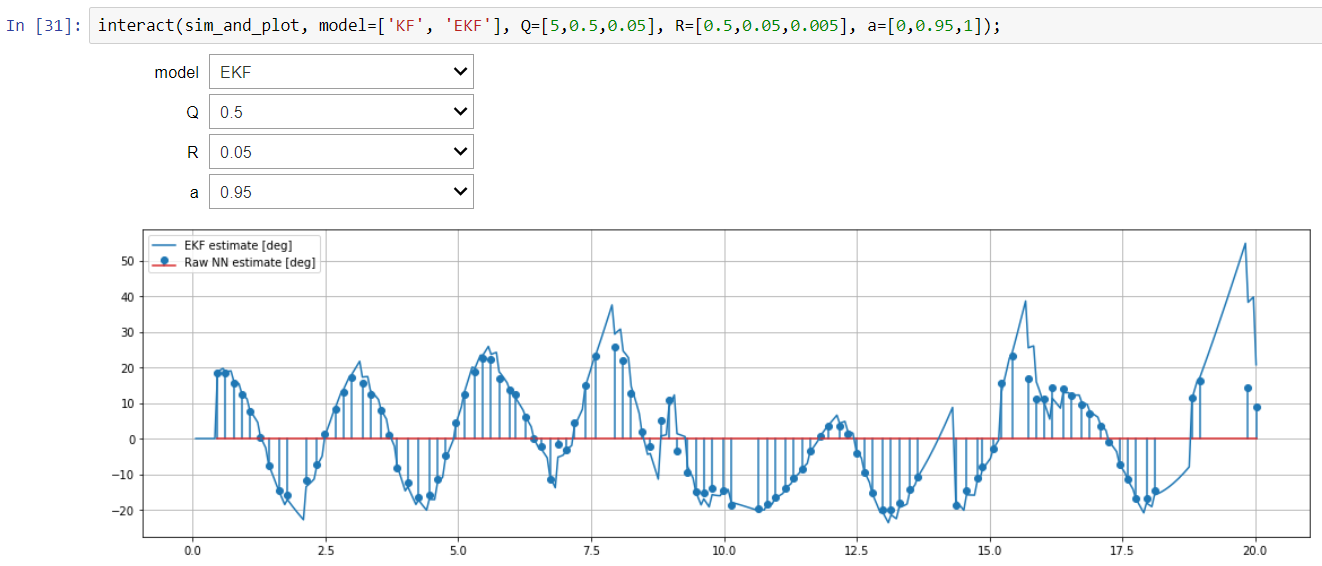
\includegraphics[width=\textwidth]{methodology/tuning_Q_R}
  \caption{\label{fig:tuning_Q_R} A plot of the output of the EKF given stem plot data as input.}
\end{figure}

As can be seen in Figure~\ref{fig:tuning_Q_R}, choosing $Q = 0.5$, $R = 0.005$ and $a = 0.95$ resulted in an EKF which closely follows and trusts the updates from the neural network, whilst making reasonable predictions in the event that no data was received. It is worth noting that the input data was more sinusoidal than 'roughly constant velocity', which was the main assumption behind the dynamics of the model. This was due to a lack of running space in the mechatronics engineering lab - once wall has been reached, there's no place to go except backwards.

\subsection{Choosing Kalman Filter or Extended Kalman Filter}\label{sec:kf_implementation}
While an EKF would be a more natural fit for the system owing to its nonlinear sensor, it was found that the linear Kalman Filter was a good option if the nonlinearity was removed by converting the pixel coordinate to an angle before passing it to the neural network. The Jacobian wasn't correct, but the filter still functioned quite well.

However, due to numerous incorrect implementations of the EKF, the linear Kalman Filter was used as part of the final system. This was mainly due to risk mitigation, as the KF was well understood while the EKF wasn't (at the time of the tests).
